\documentclass[10pt]{article}

\usepackage[margin=0.35in]{geometry}
\usepackage{multicol}
\usepackage{amsmath,amssymb,amsfonts}
\usepackage{xcolor}
\usepackage{tikz}
\usetikzlibrary{calc,arrows.meta,positioning}

% Keep typewriter usable on minimal TeX installs.
\renewcommand{\ttdefault}{cmtt}

\setlength{\parindent}{0pt}
\setlength{\parskip}{0.25em}

\begin{document}

{\Large \textbf{SEG800 Signal Cheatsheet}}\\
{\small Module 1 Week 1: \texttt{slides01\_Intro\_Signals (1).pdf} \quad | \quad Module 2 Week 2: \texttt{slides02\_Systems.pdf}}

\vspace{0.25em}
\hrule
\vspace{0.5em}

\footnotesize
\begin{multicols}{2}

\section{Signals and Systems Basics}

\textbf{Signal:} a function of one or more independent variables (e.g., time, space).\\
\textbf{System:} hardware/software device (or algorithm) that operates on an input signal to produce an output signal.\\
\textbf{Algorithm:} method/rules implementing the system's mathematical operation(s).

\section{Signal Classifications (Module 1 Week 1)}

\subsection{Continuous-Time vs.\ Discrete-Time}
\textbf{Continuous-time (analog):} defined for every real time value.\\
\textbf{Discrete-time:} defined only at specific instants (often indexed by integer $n$); undefined otherwise.\\
\textbf{Sampling:} selecting values of an analog signal at discrete times.

\subsection{Continuous-Valued vs.\ Discrete-Valued}
\textbf{Continuous-valued:} amplitude can be any real number.\\
\textbf{Discrete-valued:} amplitude limited to discrete levels (as stored/represented in a computer).\\
\textbf{Digital signal:} discrete-time + discrete-valued.\\
\textbf{Quantization:} continuous-valued $\rightarrow$ discrete-valued (e.g., rounding/truncation).

\subsection{Deterministic vs.\ Random}
\textbf{Deterministic:} uniquely described by an explicit expression, table, or well-defined rule.\\
\textbf{Random:} unpredictable/uncertain; not practically described by a simple explicit rule.

\subsection{Discrete-Time Signal Representations}
Functional form $x[n]$, tabular values, sequence notation, graphical (stem plot).

\subsection{Elementary Discrete-Time Signals}
\textbf{Unit sample (impulse):}
\[
\delta[n] =
\begin{cases}
1, & n=0\\
0, & n\neq 0
\end{cases}
\]
\textbf{Unit step:}
\[
u[n] =
\begin{cases}
1, & n\ge 0\\
0, & n<0
\end{cases}
\]
\textbf{Unit ramp:} $r[n] = n\,u[n]$.\\
\textbf{Exponential:} $x[n]=a^n$ for all $n$; causal version often appears as $a^n u[n]$.\\
Complex exponential: $x[n]=r^n e^{j\theta n}$.

\subsection{Common Time/Amplitude Operations}
\textbf{Time shift:} $x[n-k]$ (delay if $k>0$, advance if $k<0$).\\
\textbf{Folding (reflection):} $x[-n]$.\\
\textbf{Important:} folding and time shifting are \textbf{not} commutative.\\
\textbf{Down-sampling / time scaling:} $x[\mu n]$ (integer $\mu$).\\
\textbf{Amplitude ops:}
Addition: $y[n]=x_1[n]+x_2[n]$.\quad
Multiplication: $y[n]=x_1[n]x_2[n]$.\quad
Scaling: $y[n]=A\,x[n]$.

\vspace{0.25em}
\textbf{Tiny stem-plot example (time shift + fold):}
\begin{center}
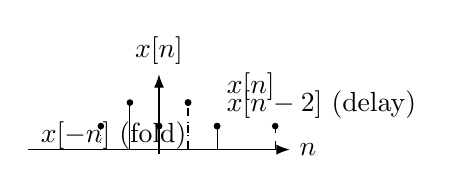
\begin{tikzpicture}[x=1.05em,y=0.85em,>=Latex,line width=0.4pt]
  % Axes
  \draw[->] (-4.5,0) -- (4.5,0) node[right] {$n$};
  \draw[->] (0,-0.2) -- (0,3.2) node[above] {$x[n]$};

  % x[n] stems (example): x[-1]=2, x[0]=1, x[2]=1
  \foreach \n/\v in {-1/2,0/1,2/1} {
    \draw (\n,0) -- (\n,\v);
    \fill (\n,\v) circle (1.2pt);
  }
  \node[anchor=west] at (2.0,2.7) {$x[n]$};

  % x[n-2] stems (delay by 2): shift right by 2
  \foreach \n/\v in {1/2,2/1,4/1} {
    \draw[dashed] (\n,0) -- (\n,\v);
    \fill (\n,\v) circle (1.2pt);
  }
  \node[anchor=west] at (2.0,1.9) {$x[n-2]$ (delay)};

  % x[-n] stems (fold)
  \foreach \n/\v in {-1/2,0/1,2/1} {
    \draw[dotted] (-\n,0) -- (-\n,\v);
    \fill (-\n,\v) circle (1.2pt);
  }
  \node[anchor=west] at (-4.4,0.6) {$x[-n]$ (fold)};
\end{tikzpicture}
\end{center}

\subsection{Energy vs.\ Power (Discrete-Time)}
\textbf{Energy:}
\[
E = \sum_{n=-\infty}^{\infty} |x[n]|^2
\]
\textbf{Average power:}
\[
P = \lim_{N\to\infty}\frac{1}{2N+1}\sum_{n=-N}^{N} |x[n]|^2
\]
\textbf{Energy signal:} $0<E<\infty$ (then $P=0$).\\
\textbf{Power signal:} $0<P<\infty$.

\subsection{Periodic vs.\ Aperiodic}
\textbf{Periodic:} $\exists N\in\mathbb{Z},\ N>0$ such that $x[n+N]=x[n]$.\\
Smallest such $N$ is the \textbf{fundamental period}.\\
Discrete-time sinusoid is periodic iff its normalized frequency is rational (as stated in the slides).

\vspace{0.25em}
\textbf{Periodic energy/power:} nonzero periodic signals are \textbf{power} signals (energy $=\infty$).\\
Average power for period $N$:
\[
P = \frac{1}{N}\sum_{n=0}^{N-1} |x[n]|^2
\]

\subsection{Even/Odd Signals and Decomposition}
\textbf{Even:} $x[n]=x[-n]$.\quad
\textbf{Odd:} $x[n]=-x[-n]$.
\[
x[n] = x_e[n] + x_o[n]
\]
\[
x_e[n] = \frac{x[n] + x[-n]}{2},
\qquad
x_o[n] = \frac{x[n] - x[-n]}{2}
\]

\section{Discrete-Time Systems (Module 2 Week 2)}

\textbf{Discrete-time system:} maps input $x[n]$ to output $y[n]$ via a rule:
\[
y[n] = T\{x[n]\}
\]

\subsection{Basic System Blocks}
Adder: $y[n]=x_1[n]+x_2[n]$.\\
Constant multiplier: $y[n]=a\,x[n]$.\\
Signal multiplier: $y[n]=x_1[n]x_2[n]$.\\
Unit delay: $y[n]=x[n-1]$.\\
Unit advance: $y[n]=x[n+1]$.\\
Accumulator: $y[n]=y[n-1]+x[n]$.\\
\textbf{Initially relaxed:} system has zero initial condition / stored state, e.g., $y[n_0]=0$.

\vspace{0.25em}
\textbf{Block diagram symbols (common):}
\begin{center}
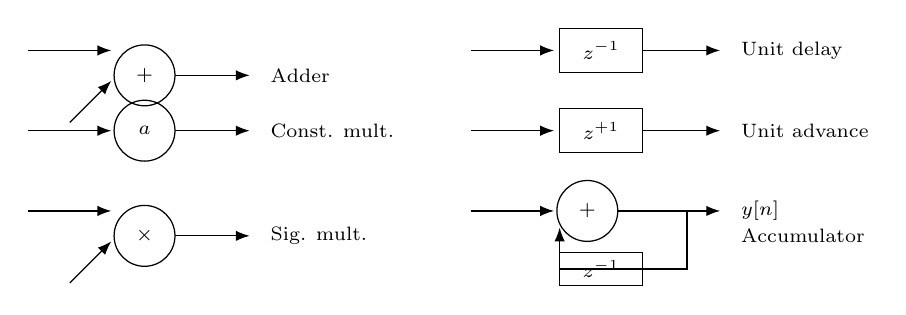
\begin{tikzpicture}[x=1em,y=1em,>=Latex,line width=0.45pt,every node/.style={font=\scriptsize}]
  % Layout anchors
  \coordinate (L0) at (0,6);
  \coordinate (R0) at (16,6);

  % --- Adder ---
  \draw[->] ($(L0)+(0,0)$) -- ($(L0)+(3,0)$);
  \draw[->] ($(L0)+(1.5,-2.6)$) -- ($(L0)+(3,-1.1)$);
  \draw ($(L0)+(4.2,-0.9)$) circle (1.1);
  \node at ($(L0)+(4.2,-0.9)$) {$+$};
  \draw[->] ($(L0)+(5.3,-0.9)$) -- ($(L0)+(8,-0.9)$);
  \node[anchor=west] at ($(L0)+(8.4,-0.9)$) {Adder};

  % --- Constant multiplier ---
  \coordinate (L1) at (0,3.1);
  \draw[->] ($(L1)+(0,0)$) -- ($(L1)+(3,0)$);
  \draw ($(L1)+(4.2,0)$) circle (1.1);
  \node at ($(L1)+(4.2,0)$) {$a$};
  \draw[->] ($(L1)+(5.3,0)$) -- ($(L1)+(8,0)$);
  \node[anchor=west] at ($(L1)+(8.4,0)$) {Const. mult.};

  % --- Signal multiplier ---
  \coordinate (L2) at (0,0.2);
  \draw[->] ($(L2)+(0,0)$) -- ($(L2)+(3,0)$);
  \draw[->] ($(L2)+(1.5,-2.6)$) -- ($(L2)+(3,-1.1)$);
  \draw ($(L2)+(4.2,-0.9)$) circle (1.1);
  \node at ($(L2)+(4.2,-0.9)$) {$\times$};
  \draw[->] ($(L2)+(5.3,-0.9)$) -- ($(L2)+(8,-0.9)$);
  \node[anchor=west] at ($(L2)+(8.4,-0.9)$) {Sig. mult.};

  % --- Unit delay ---
  \coordinate (R1) at (16,6);
  \draw[->] ($(R1)+(0,0)$) -- ($(R1)+(3,0)$);
  \draw ($(R1)+(3.2,-0.8)$) rectangle ($(R1)+(6.2,0.8)$);
  \node at ($(R1)+(4.7,0)$) {$z^{-1}$};
  \draw[->] ($(R1)+(6.2,0)$) -- ($(R1)+(9,0)$);
  \node[anchor=west] at ($(R1)+(9.4,0)$) {Unit delay};

  % --- Unit advance ---
  \coordinate (R2) at (16,3.1);
  \draw[->] ($(R2)+(0,0)$) -- ($(R2)+(3,0)$);
  \draw ($(R2)+(3.2,-0.8)$) rectangle ($(R2)+(6.2,0.8)$);
  \node at ($(R2)+(4.7,0)$) {$z^{+1}$};
  \draw[->] ($(R2)+(6.2,0)$) -- ($(R2)+(9,0)$);
  \node[anchor=west] at ($(R2)+(9.4,0)$) {Unit advance};

  % --- Accumulator y[n] = y[n-1] + x[n] ---
  \coordinate (R3) at (16,0.2);
  % input x[n]
  \draw[->] ($(R3)+(0,0)$) -- ($(R3)+(3,0)$);
  % adder
  \draw ($(R3)+(4.2,0)$) circle (1.1);
  \node at ($(R3)+(4.2,0)$) {$+$};
  \draw[->] ($(R3)+(5.3,0)$) -- ($(R3)+(9,0)$);
  \node[anchor=west] at ($(R3)+(9.4,0)$) {$y[n]$};
  % feedback through delay
  \draw ($(R3)+(7.8,0)$) |- ($(R3)+(7.8,-2.1)$) -- ($(R3)+(3.2,-2.1)$);
  \draw ($(R3)+(3.2,-2.7)$) rectangle ($(R3)+(6.2,-1.5)$);
  \node at ($(R3)+(4.7,-2.1)$) {$z^{-1}$};
  \draw[->] ($(R3)+(3.2,-2.1)$) -- ($(R3)+(3.2,-0.6)$);
  \node[anchor=west] at ($(R3)+(9.4,-0.9)$) {Accumulator};
\end{tikzpicture}
\end{center}

\subsection{System Classification Checklist}
\textbf{Memoryless (static):} $y[n]$ depends only on $x[n]$.
Often written as $y[n]=T\{x[n],n\}$.\\
\textbf{Dynamic:} depends on past/future samples (has memory).
Finite memory (duration $N$): depends only on $\{x[n],x[n-1],\ldots,x[n-N]\}$.
Infinite memory: otherwise.
Depending on future samples requires a stored signal (not physically realizable in real-time).\\
\textbf{Time-invariant (initially relaxed):} for \emph{every} input $x[n]$ and \emph{every} integer shift $k$,
\[
T\{x[n-k]\} = y[n-k]
\]
\textbf{Linear (superposition):} for constants $a,b$,
\[
T\{a x_1[n] + b x_2[n]\} = aT\{x_1[n]\} + bT\{x_2[n]\}
\]
Scaling: $T\{a x[n]\}=aT\{x[n]\}$.\quad Additive: $T\{x_1[n]+x_2[n]\}=T\{x_1[n]\}+T\{x_2[n]\}$.\\
\textbf{Causal:} depends only on present/past inputs.
Often written $y[n]=F(x[n],x[n-1],x[n-2],\ldots)$.\\
\textbf{BIBO stable:} if $|x[n]|\le M_x<\infty$ for all $n$, then $|y[n]|\le M_y<\infty$ for all $n$.

\subsection{Interconnection of Discrete-Time Systems}
\textbf{Cascade (series):} $y_1[n]=T_1\{x[n]\}$, $y[n]=T_2\{y_1[n]\}=T_2\{T_1\{x[n]\}\}=(T_2\circ T_1)\{x[n]\}$.\\
\textbf{Parallel:} $y[n]=y_1[n]+y_2[n]=T_1\{x[n]\}+T_2\{x[n]\}$.

\section{LTI Systems and Convolution (Module 2 Week 2)}

\subsection{Impulse Resolution of a Sequence}
Any discrete-time signal can be expressed as a weighted sum of shifted impulses:
\[
x[n] = \sum_{k=-\infty}^{\infty} x[k]\,\delta[n-k]
\]

\subsection{Impulse Response and Convolution Sum}
For LTI systems, define impulse response:
\[
h[n] = T\{\delta[n]\}
\]
Then the output is:
\[
y[n] = (x*h)[n] = \sum_{k=-\infty}^{\infty} x[k]\,h[n-k]
\]

\textbf{Where convolution comes from:} impulse decomposition + superposition (linearity) + time invariance.

\subsection{Manual Convolution Procedure}
Folding (time-reverse), shifting, multiplication, summation (choose the easier sequence to fold).\\
\textbf{Commutative:} $x*h = h*x$.

\subsection{Convolution Properties (LTI)}
Identity: $x[n]*\delta[n]=x[n]$.\\
Shift: $x[n]*\delta[n-n_0]=x[n-n_0]$.\\
Commutative: $x*h=h*x$.\\
Associative: $(x*h_1)*h_2 = x*(h_1*h_2)$.\\
Distributive: $x*(h_1+h_2) = x*h_1 + x*h_2$.

\subsection{Causality and Stability via $h[n]$}
LTI causal $\Leftrightarrow h[n]=0$ for $n<0$.\\
Initially relaxed LTI BIBO stable $\Leftrightarrow$ $h[n]$ is absolutely summable:
\[
\sum_{n=-\infty}^{\infty} |h[n]| < \infty
\]

\section{FIR vs.\ IIR and Difference Equations (Module 2 Week 2)}

\textbf{FIR:} finite-duration impulse response (finite memory).\\
\textbf{IIR:} infinite-duration impulse response (often due to feedback; infinite memory).\\
Difference equations are commonly used to represent LTI systems (especially IIR).

\subsection{General Difference Equation (LTI)}
\[
y[n]= -\sum_{k=1}^{N} a_k\,y[n-k] + \sum_{k=0}^{M} b_k\,x[n-k]
\]
FIR: $a_k=0$ (no feedback).\quad IIR: some $a_k\neq 0$ (feedback).

\section{Smoothing Filters Mentioned (Module 2 Week 2)}

\textbf{Causal moving average (MA), length $M$:}
\[
y[n] = \frac{1}{M}\sum_{k=0}^{M-1} x[n-k]
\]
\textbf{Symmetric moving average (SMA):} non-causal (uses future samples).\\
\textbf{First-order exponential smoothing (typical form):}
\[
y[n] = a\,y[n-1] + (1-a)\,x[n]
\]
(slides note $b=1-a$).

\end{multicols}
\end{document}
